\title{Представление данных для сборки мусора}
%
\titlerunning{Представление данных для сборки мусора}
\author{Крень Мария Владимировна}
%
\authorrunning{М.В.Крень} % abbreviated author list (for running head)
%
%%%% list of authors for the TOC (use if author list has to be modified)
\tocauthor{М.В.Крень}
%
\institute{Санкт-Петербургский государственный университет\\
\email{mari.kren@gmail.com}}

\maketitle              % typeset the title of the contribution

\begin{abstract}
В работе рассматриваются несколько моделей представления объектов
в памяти, которые обеспечивают решение основных задач, возникающих
при сборке мусора.
\end{abstract}
%

\section*{Введение}

\emph{Сборка мусора} --- это один из способов автоматического управления динамической памятью.
Суть сборки мусора заключается в том, что память, которая в дальнейшем не понадобится, освобождается системой управления памятью автоматически. 
Для этого иногда запускается процесс, называемый сборкой  мусора.
Поскольку, в общем случае, невозможно точно определить момент, когда объект использован в последний раз и
больше не нужен, сборщики мусора используют для этого консервативную оценку.
В качестве такой оценки используется понятие достижимости объекта из достижимых объектов. 
Начальное множество достижимых объектов определяется аксиоматически в зависимости от платформы.

Сборка мусора обладает как достоинствами, так и недостатками.
По сравнению с ручным управлением, автоматическое управление памятью безопаснее: программисту не нужно 
заботиться о том, когда освобождать память из-под объектов. 
Это дает гарантию того, что не возникнет некоторых ошибок, таких как
висячий указатель, то есть указатель на уже освобожденный объект, или ошибка повторного освобождения памяти, 
когда программа пытается освободить память, которая уже  была освобождена.
При интенсивном выделении и освобождении памяти может возникнуть ситуация,
когда непрерывный блок памяти определенного размера не может быть выделен,
хотя суммарный объем свободной памяти вполне достаточен. Сборка мусора часто позволяет избежать такой
ситуации за счет перемещения объектов и уплотнения занятой ими области.

С другой стороны при автоматическом управлении памятью могут возникнуть следующие проблемы:
\begin{enumerate}
\item Если на объект есть ссылки из других достижимых объектов, то он никогда не будет удален.
\item Во время работы программы из-за работы сборщика мусора возникают паузы в случайные моменты времени, а их продолжительность не определена.
Помимо этого, приходится затрачивать время на отслеживание дополнительной информации по объектам.
\item Должны быть выполнены  требования для реализации сборщика мусора.
Во-первых, должна присутствовать возможность определить все указатели из любого объекта на другие элементы кучи.
Во-вторых, не должно быть никаких операций над указателями (логических, арифметических и т.п.)
\end{enumerate}

Целью данной работы являются изучение существующих наиболее используемых моделей представления данных для сборки мусора и
разработка библиотеки, реализующей типичную модель.

\section{Обзор существующих реализаций}

Параметрический и объектный полиморфизм, свойственные современным языкам программирования, требуют единообразного представления  
значения различных типов. С этой целью все представления разбиваются на два класса: ``boxed'' и ``unboxed''. ``Boxed''--значение представляет 
собой ссылку на соответствующее значение в куче, а доступ к ``unboxed''--значению осуществляется напрямую. 
Сборщику мусора надо уметь отличать эти представления друг от друга и находить указатели внутри любого из них.

Основной подход к решению данной проблемы --- хранение метаданных. Самым простым примером метаданных являются теги.
Обычно выделяется несколько бит (меньшая часть машинного слова) под кодировку информации о типе. Например, интерпретатор GNU Еmacs Lisp 
поддерживает 24-битные целые несмотря на то, что машинное целое 32-битное. Восемь бит используется для хранения информации о типе,
необходимой интерпретатору.

Далее представлен обзор некоторых моделей представления данных.

\subsection {Java Virtual Machine(JVM)}

JVM (Java Virtual Machine, виртуальная машина Java)\footnote{http://docs.oracle.com/javase/specs/jvms/se7/html/index.html}
является основной частью исполняющей системы Java, так называемой Java Runtime Environment (JRE).
JVM исполняет байт-код, предварительно созданный из исходного текста программы компилятором, а также
предоставляет ей всю поддержку времени исполнения, включая управление памятью и сборку мусора.

Все типы JVM разделяются на два класса --- \emph{примитивные} (primitive) и \emph{ссылочные} (reference).
Значения примитивных типов представляются в виде unboxed--последовательности из одного или более машинных слов.
Ссылочные типы представляются указателем в кучу. Разделение на примитивные и ссылочные типы является статическим.

Значение ссылочного типа представляется в виде \emph{объекта}.
Каждый объект содержит заголовок\footnote{http://jug.ua/wp-content/uploads/2013/02}, который для 
большинства JVM (Hotspot, openJVM) состоит из двух или трех машинных слов.

Структура заголовка:

\begin{itemize}
\item Mark Word --- содержит хэш--код объекта, информацию для системы управления памятью, информацию о состоянии блокировки. 
\item Type Information Block Pointer (TIBP) --- содержит информацию о типе объекта в виде указателя на экземпляр класса Class.
\item Array Length --- длина массива (только если объект является массивом).
\end{itemize}            

Чтобы отличить указатель от не указателя, нужно из TIBP получить методом getType тип объекта\footnote{http://docs.oracle.com/javase/6/docs/api/java/lang/Class.html}.

\subsection {Parallel Haskell compiler}

Parallel Haskell compiler (pHc)~\cite{pHc} — компилятор для языка Haskell.
<<<<<<< .mine
Как известно, Haskell -- язык программирования со строгой, статической типизацией и автоматическим выводом типов.
При строгой типизации данных в языке, подходы к определению типов отличаются от подходов при динамической типизаци и хранение ранее упомянутых тегов для умения отличать ''boxed''-значения от ''unboxed'' необязательно.
Рассмотрим 64-битную модель представления данных для pHc, которая позволяет эффективно, с использованием минимального количества памяти под тег различать типы.
Это достигается за счет того, что информация, которую обычно содержит большая часть тега, кодируется с гораздо меньшим негативным влиянием на диапазон данных / точность и не использует для кодирования дополнительной памяти.
От тегов не отказываются, но область памяти, отводимая под них, минимизируется.

=======
При строгой типизации данных в языке, подходы к определению типов отличаются от подходов при динамической типизации.
Как известно, Haskell -- язык программирования со строгой, статической типизацией и автоматическим выводом типов.
Рассмотрим 64-битную модель представления данных для pHc, которая позволяет эффективно, с использованием минимального количества памяти под тег различать типы.
Это достигается за счет того, что информация, которую обычно содержит большая часть тега, кодируется с гораздо меньшим негативным влиянием на диапазон данных / точность и не использует для кодирования дополнительной памяти.
От тегов не отказываются, но область памяти, отводимая под них, минимизируется.

>>>>>>> .r56
Рассмотрим модели данных в pHc.

Integers/pointer bit --- модель, каждый образец которой --- знаковое целое 64-битной ширины, 
во многих случаях являющееся также указателем.

Floating point bit --- модель, образец которой --- число с плавающей точкой 64-битной ширины стандарта IEEEE-754.

Если значение объекта меньше чем 0х8FF0..., тогда это либо целое число, либо число с плавающей точкой,
иначе это указатель.

Минусы такого представления данных: 
\begin{enumerate}
\item неэффективная арифметика (из-за размеров целых чисел);
\item если происходит необработанное переполнение, то интерпретатор может 
подумать, что это указатель, а не отрицательное число.
\end{enumerate}

\subsection {Guile}

Guile\footnote{http://www.gnu.org/software/guile/manual} --- интерпретатор и компилятор для языка Sсheme, который
является языком с динамической типизацией.

%Язык Scheme\footnote{cs.princeton.edu/picasso/mats} динамически типизирован.
%Т.е. система не может определить тип данного выражения во время компиляции, тип может быть определен только во время выполнения.
%Переменные в Scheme не имеют фиксированных типов, т.е. могут быть
%типа ``пара'' в один момент времени, потом целочисленного типа, а потом ``вектором'' из тысячи элементов. Значения
%имеют фиксированный тип. Представление каждого значения должно содержать достаточно
%информации для точного определения типа во время выполнения.

%Из-за переменных ``пар'' и ``векторов'', которые могут хранить значения любых типов,

В реализации Scheme использовано общее представление для значений ---
один ``большой'' тип, которого достаточно для хранения значения или указателя на значение,
перед которыми идет необходимая информация о типе. Самый простой способ описать такое значение в терминах С --- 
это сделать его указателем на структуру, содержащую идентификатор типа, а после него объединение 
значений:

\begin{lstlisting}
enum type { integer, pair, string, vector, ... };
  
typedef struct value *SCM;
  
struct value {
  enum type type;
  union {
    int integer;
    struct { SCM car, cdr; } pair;
    struct { int length; char *elts; } string;
    struct { int length; SCM  *elts; } vector;
    ...
  } value;
};
\end{lstlisting}

Обратившись к полю \texttt{type} в структуре, можно отличить указатель от не указателя.

\subsection {CHICKEN}

CHICKEN --- это компилятор для языка Scheme. В реализации CHIСKEN использован довольно простой и эффективный метод представления данных.
Под метаданные резервируется несколько битов слова. Для этих битов существуют коды, которые отвечают за
принадлежность объектов к различным моделям представления. Коды хранят специальную информацию о состоянии объектов.
В  модели представления данных данного компилятора
существует два вида объектов: immediate и non--immediate.

\begin{enumerate}
\item Immediate--объекты.
Объекты данного типа либо 32-битной, либо 64-битной ширины, в зависимости от архитектуры.
\item Fixnums --- самый маленький точный integer, в котором младший порядковый бит 
установлен 1, остальные 31 бит или 63 бита остаются под значение.
\item Characters --- здесь 4 младших бита 1010, 24 последующие бита под данные.
\item Booleans --- последние 4 бита --- 0110, а 5-й --- 1, если true, 0 --- false.
\item Другие значения --- последние 4 бита 1110, следующие четыре кодируют одно из значений:
\begin{itemize}
\item \lstinline{C_SCHEME_END_OF_LIST} --- 0000;
\item \lstinline{C_SCHEME_UNDEFINED} --- 0001;
\item \lstinline{C_SCHEME_UNBOUND} --- 0010;
\item \lstinline{C_SCHEME_END_OF_FILE} --- 0011.
\end{itemize}

\item Non-immediate--объекты.
Это блоки данных, представленные указателями в куче.
Первое слово блока данных содержит заголовок, оно дает информацию о типе объекта. 
Двадцать четыре младших бита заголовка хранят длину данного объекта.
Четыре старших бита заголовка используется для сборки 
мусора.
После этих четырех бит идут следующие четыре, представляющие собой один из 15 типов или специальную метку.
\end{enumerate}

В данной модели представления данных два младших бита отвечают за принадлежность объекта к той или иной 
группе. Например, если самый младший бит и следующий за ним равны единице, то это объект типа fixnum.
Когда помечен только следующий после младшего бит, то это объект типа non-immediate.
Таким образом, отличить указатель от не указателя в данной модели мы можем за одну 
операцию\footnote{http://wiki.call-cc.org/man}.

\subsection {OСaml}

OCaml\footnote{http://caml.inria.fr} --- современный объектно-ориентированный язык функционального программирования общего назначения. 
Инструментарий OCaml включает в себя интерпретатор, компиляторы в байткод и машинный код.
Каждое значение в OCaml является либо целым, либо указателем.
Два младших бита указателя всегда 0 для 32-битной системы, для 64-битной 3 младших бита всегда 0. У целых младший бит --- 1. 
Таким образом отличить целое от указателя можно за одну операцию.

Объекты больше или более сложные, чем простое целое, хранятся в OСaml в блоках.
Блок в OCaml состоит из заголовка и массива слов. Слово содержит 4 или 8 байт, это зависит от разрядности платформы.
Если значение --- указатель на блок, тогда этот указатель указывает на 0-й элемент массива, а
заголовок --- это отрицательное смещение указателя на 4 или 8 байт.
Строка в OCaml хранится, как массив байт,
с достаточным количеством слов, выделяемых для требуемого размера строки.
Массив хранится, как массив значений,
каждое слово соответствует одному значению.

Заголовок в OCaml представляет из себя:
\begin{enumerate}
\item Количество слов в блоке, например, длину массива. Для 32--разрядных систем эта часть занимает в заголовке 22 бита.
\item Далее идет тег, который используется для определения того, что эта строка содержит информацию для сборки мусора\footnote{http://rwmj.wordpress.com/2009/08/04/ocaml-internals}.
\end{enumerate}
 
\section {Проделанная работа}

В данном разделе описывается прототип модели представления данных, подходящий для представления объектов в языках со статической типизацией.
Модель построена на основе существующих моделей, некоторые из которых были представлены в обзоре. Можно заметить, что ряд компиляторов используют модели, схожие с 
представленными ниже. Например, в моделях JVM есть заголовок и значение, и во всех ниже представленных моделях есть заголовок. В представлении массивов в JVM 
используются смещения указателей, как и в этой работе, но для хранения указателей в структурах.  Как и в CHIСKEN, использованы теги для нумерации моделей,
а простейшие объекты представлены похожим образом. В представленном ниже описании будем считать, что ``unboxed''--объект --- это объект,
вмещающийся в одно машиннное слово \lstinline{word_t}.  Никакой информации о сущности такого объекта, кроме его значения, мы получить не можем.
Объект является ``boxed'', если он принадлежит одному из пяти типов моделей, описанных ниже, или на его хранение требуется больше,
чем одно машинное слово.

Рассмотрим модели (Рис.~\ref{first}). Первые три модели (Model\_4, Model\_3, Model\_2) имеют общую структуру, различающуюся лишь тегом и типом хранимых объектов.

Структура:
\begin{enumerate}
\item Поле \lstinline{TAG} --- хранит в себе номер модели. Размер тега --- 3 бита, данный размер выбран из-за количества моделей (5).
\item Поле \lstinline{SIZE} --- хранит в себе количество слов в объекте. Размер в памяти, отводимый для \lstinline{SIZE}, зависит от размера машинного слова и вычисляется как \lstinline{sizeof(word_t-3)}.
\item Массив слов --- хранит данные, тип которых определяется моделью.
\end{enumerate}

\begin{figure}[h]
%\centering
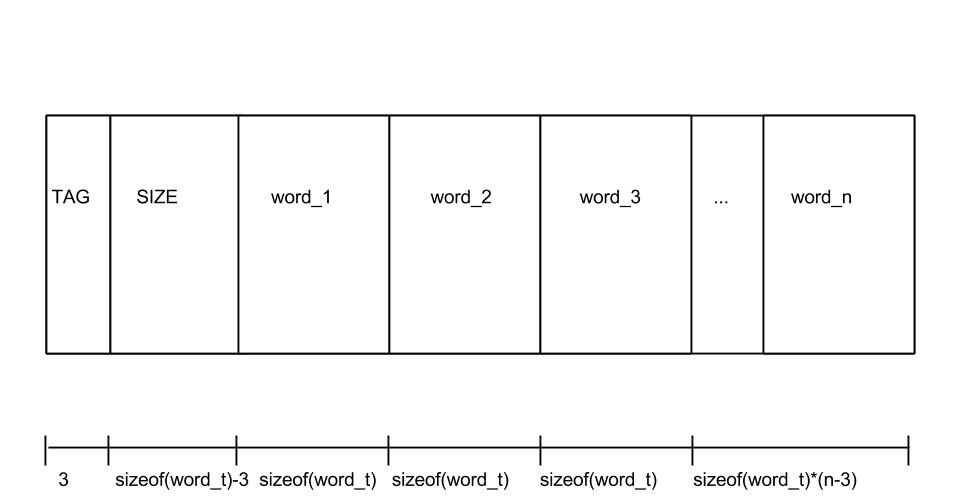
\includegraphics[width=0.65\textwidth]{Kren/1}
\caption{структура первых трех моделей}
\label{first}
\end{figure}

\begin{itemize}
\item Model\_4 --- массив указателей на ``unboxed''--значения, помещающиеся в одно слово.
Тег у данной модели равен 100.
\item Model\_3 --- массив указателей на ``boxed''--значения.
Тег у данной модели равен 100.

\item Model\_2 --- объект без указателей, хранит массив ``unboxed''--значений.
Тег у данной модели равен 010.

\item Model\_1 --- объект, расположение и тип указателей в котором представлены массивом смещений(Рис.~\ref{srcond}):
\begin{enumerate}
\item Поле \lstinline{TAG} --- такой же, как и в предыдущих трех моделях. Значение тега равно 001.
\item Поле \lstinline{SIZE} --- такой же, как и в предыдущих трех моделях.
\item Поле \lstinline{N} --- один байт отводится на хранение количества указателей.
\item \lstinline{N} ячеек --- смещение указателя и метка (указатель на ``unboxed''-- или ``boxed''--значение), каждая ячейка размера \lstinline{sizeof(word_t)}, где 1 бит отводится под метку). 
\item Cлова с данными занимают размер \lstinline{SIZE * sizeof (word_t)}.
\end{enumerate}

\begin{figure}[h]
%\centering
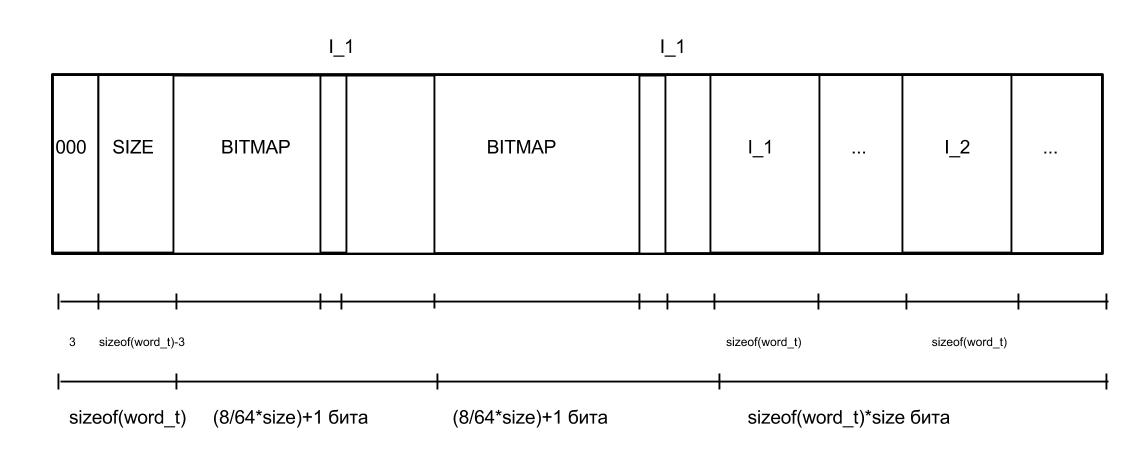
\includegraphics[width=1\textwidth]{Kren/2}
\caption{Model\_1}
\label{second}
\end{figure}

\item Model\_0 --- объект, расположение и тип указателей в котором представлены битовыми картами (Рис.~\ref{third}):
\begin{enumerate}
\item \lstinline{TAG} --- такой же, как и в предыдущих четырех моделях. Значение тега равно 000.
\item \lstinline{SIZE} --- такой же, как и в предыдущих четырех моделях.
\item Два битовых массива ---  каждый из которых размером: \lstinline{(8(sizeof(byte))/64(sizeof(word_t)))/ * SIZE) + 1}, в одном массиве хранятся смещения указателей, во втором метка (указатель на ``uboxed''-- или ``boxed''--значение).
\item Cлова с данными --- занимают размер \lstinline{SIZE * sizeof (word_t)}.
\end{enumerate}
Смещения указателей записаны в битовый массив следующим образом: \lstinline{ptr.offset - (ptr.offset/CHAR_BIT) * CHAR_BIT};
метка записывается, как и смещение.
\end{itemize}
\begin{figure}[h]
%\centering
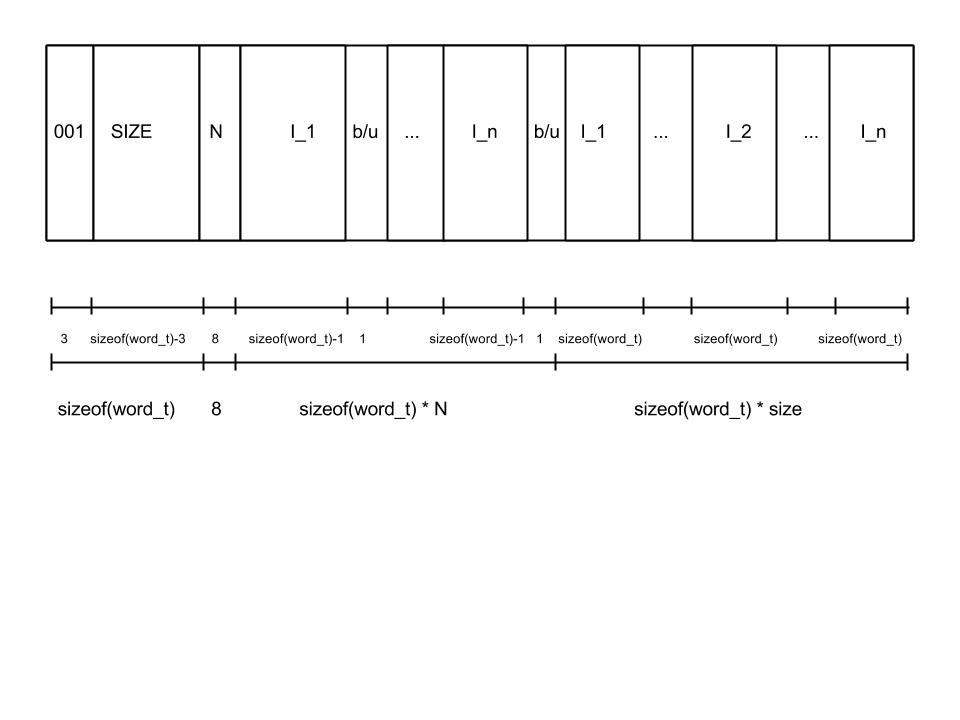
\includegraphics[width=0.8\textwidth]{Kren/3}
\caption{Model\_0}
\label{third}
\end{figure}

Функции для работы с моделями:
\begin{enumerate}
\item \lstinline{size_t get_size(void * object)} --- возвращает количество не пустых слов объекта; 
\item \lstinline{word_t get_word(void * object, size_t index)} --- возвращает слово;
\item \lstinline{void * get_ptr (void * object, size_t index)} --- возвращает указатель на слово;
\item \lstinline{void   set_word(void * object, size_t index, word_t data)} --- записывает данные в слово;
\item \lstinline{void   set_ptr (void * object, size_t index, void* data)} --- записывает указатель;
\item \lstinline{PTR_ITERATOR get_iterator (void * object)} --- создает итератор по указателям данного объекта;
\item \lstinline{void * next_ptr(PTR_ITERATOR * iterator)} --- получает следующий указатель.
\end{enumerate}
Такое представление данных позволит нам за минимальное число операций различать объекты, совершать над ними примитивные операции.


\section{Пример}
В данной секции описывается пример использования вышеописанных моделей данных.
В примере создаются списки рабочих, каждому из которых сопоставляется список клиентов. Реализован оператор выбора клиентов на указанную букву,  для списка рабочих.
Полный перечень основных функций: функция добавления клиента в список клиентов \lstinline{add_client}, добавления рабочих в список рабочих \lstinline{add_workers}, 
функции печати (\lstinline{print_list_workers}, \lstinline{print_list_clients}) списков и функция выбора (\lstinline{select_client}),
возвращающая из заданного числа списков рабочих,  всех клиентов с именами на заданную букву.  

\begin{lstlisting}[mathescape]
# include <stdio.h>
# include <prototype.h>

// $\mbox{функция с переменным числом аргументов, записывающая рабочих в структуру;}$
// $\mbox{имя рабочего записывается в паре с его идентификационным номером}$
// $\mbox{параметры функции: структура, хранящая рабочих и идекс рабочего,}$
// $\mbox{количество добавляемых рабочих, имена}$

void  add_workers(void * list,int count, ...) { 
  va_list args;                                 
  va_start (args, count);
  // $\mbox{счетчик для итераций по всем словам структуры}$
  size_t i = 1;
  // $\mbox{счетчик для итераций с пустого слова структуры}$
  size_t j = 1;
  // $\mbox{количество непустых слов в структуре с рабочими}$
  size_t len = get_size(list);
  if (count != 0) // $\mbox{если введено не ноль имен}$
  {
    // $\mbox{нахождение первого свободного слова в структуре}$
    for ( ; j < len + 1; j++) {  
      if ( get_word(list, j) == 0)  
      break;
    }
    if( j == len) {  // $\mbox{случай, когда возвращается индекс последнего слова}$
      return;        // $\mbox{без записи}$
    }
    else {  // $\mbox{случай, когда есть свободные ячейки}$
        // $\mbox{запись индекса и имени работника \texttt{count} раз}$
        for ( ; i < (size_t)(count+1); i++) {
          // $\mbox{берется следующее имя из параметров функции}$
          char * namels = va_arg(args, char *);
          // $\mbox{выделение памяти под объект с именем}$
          void * name = create_generic_object(strlen(namels), 0);  
          create_name(namels,name);  // $\mbox{запись имени в объект}$
          // $\mbox{запись индекса рабочего в структуру с рабочими}$
          set_word(list, j, (j+1)/2 );
          // $\mbox{запись указателя на объект с именем рабочего}$
          set_ptr(list, j+1, name);  
          j+=2;  // $\mbox{индекс увеличивается на 2 из-за попарного заполнения слов}$
         }
        }
  }
  return;
}
// $\mbox{функция записи имени в объект}$
void  create_name(char * name, void * res) {  // $\mbox{параметры: имя, объект}$
  size_t len = strlen(name); // $\mbox{вычисляется длина имени}$
  size_t i = 1;  // $\mbox{создается итератор по имени}$
  for (; i < len + 1; i++) {
    set_word(res, i, name[i-1]);  
    // $\mbox{итерации по имени и запись символов в объект}$
  }
  return;
}

// $\mbox{функция с переменным числом аргументов, записывающая клиентов в ``boxed''--массив;}$
// $\mbox{параметры функции: массив, хранящий указатели на объекты с именами клиентов,}$
// $\mbox{количество добавляемых клиентов, их имена}$
void  add_client(void * list, size_t count, ...) {
    va_list args;
    va_start (args, count);
    // $\mbox{счетчик для итераций по всем словам массива}$
    size_t i = 1;
    // $\mbox{счетчик для итераций с пустого слова массива}$
    size_t j = 1;
    // $\mbox{количество непустых слов в массиве с клиентами}$
    size_t len = get_size(list);
    if (count != 0)  // $\mbox{если введено не нуль имен}$
    {
        // $\mbox{нахождение первого свободного слова в массиве}$
        for ( ; j < len + 1; j++) { 
            if (get_word(list, j) == 0)
               break;
        }
        if( j == len) {  // $\mbox{случай, когда возвращается индекс последнего слова}$
          return;        // $\mbox{без записи}$
        }
        else {  // $\mbox{случай, когда есть свободные ячейки}$
                // $\mbox{запись имени работника count раз}$
            for ( ; i < (size_t)(count+1); i++) {
              // $\mbox{берется следующее имя из параметров функции}$
              char * namels = va_arg(args, char *);
              // $\mbox{выделение памяти под объект с именем}$
              void * name = create_generic_object(strlen(namels), 0);  
              create_name(namels,name);  // $\mbox{запись имени в объект}$
              // $\mbox{запись указателя на объект с именем клиента}$
              set_ptr(list, j, name);
              j++;
           }
          }
    }
    return;
}

// $\mbox{функция с переменным числом аргументов, выполняющая выборку клинтов;}$
// $\mbox{выборка производится из массива ``boxed''--указателей на списки клиентов}$
// $\mbox{первых \texttt{count}--рабочих, по букве \texttt{ch}}$
void * select_client(void * list_client_allworkers,
                     char ch, size_t count, ...)  {  
  va_list args;
  va_start (args, count);
  void * list_cl;  
  // $\mbox{результирующий массив ``boxed''--указателей на объекты с именами}$
  size_t all_num = 0;  // $\mbox{количество клиентов на заданную букву}$
  size_t i = 1;  // $\mbox{итератор по всем спискам клиентов}$
  size_t past = 1;  // $\mbox{счетчик записей имен}$
  for ( ; i < count + 1; i++) {
    // $\mbox{возвращает количество имен на букву \texttt{ch} из списка клиентов рабочего с таким \texttt{id}}$
    all_num += get_num_name(list_client_allworkers, i, ch);   
  }
  list_cl = create_boxed_array(all_num);  // $\mbox{выделяется память под массив}$
  i = 1;
  for ( ; i < count + 1; i++) {
    // $\mbox{запись указателей на объекты с нужными именами}$
    past = paste_name(list_cl, list_client_allworkers, i, past, ch);
  }
  return list_cl;
}

// $\mbox{возвращает количество имен на букву \texttt{let} из списка клиентов рабочего с таким \texttt{id}}$
size_t get_num_name(void * list_client_allworkers, size_t id, char let) {
void * ls_i = ((void *)get_word(list_client_allworkers, id));
size_t count = get_size(ls_i);
size_t i = 1;
size_t j = 0;
void * tmp;
      for (; i < count + 1; i++) {
          tmp = (void *)get_word(ls_i, i);
    if ( start_letter(tmp, let) == 1) {
      j++;
	}
      }
return j;
}

// $\mbox{функция сравнивает первую букву объекта и заданную let}$
size_t start_letter(void * obj, char  let) {
    if ( get_word(obj, 1) == (word_t)let)
    return 1;
  return 0;
}
// $\mbox{функция записывает в \texttt{list\_cl} клиентов на заданную букву \texttt{let} и}$
// $\mbox{возвращает количество сделаных записей;}$
// $\mbox{аргументы: результирующий массив, массив клиентов, индекс клиента, буква}$
size_t paste_name(void * list_cl, void * list, size_t n,
size_t j, char let) {
void * ls_i = (void *)get_word(list,n);
size_t count = get_size(ls_i);
size_t i = 1;
for (; i < count + 1; i++) {
  if (start_letter( (void *)get_word(ls_i, i), let) == 1) {
    set_word(list_cl, j, get_word(ls_i, i));
    j++;
  }
}
return j;
}

// $\mbox{функция печати списка рабочих c индентификатором}$
void print_list_workers(void * list) {
    size_t len = get_size(list);
    size_t len2;
    void * nam1;
    size_t i = 2;
    size_t j ;
    word_t tmp;
    for (; i < (size_t)(len+1); i += 2) {
        tmp = get_word(list, i-1);
        printf("$\mbox{работник:}$ " "%i ", (int)tmp);
        nam1 = (void *)get_word(list, i);
        if (nam1 != 0){
            len2 = get_size(nam1);
            for (j = 1; j < len2+1; j++) {
                tmp = get_word(nam1, j);
                printf("%c", tmp, tmp);
            }
            printf("\n");
        }
    }
}
// $\mbox{функция печати списка клиентов}$
void print_list_clients(void * list) {
    size_t len = get_size(list);
    size_t len2;
    void * nam1;
    size_t i = 1;
    size_t j;
    word_t tmp;
    for (; i< len+1; i++) {
        nam1 = (void *)get_word(list, i);
        if (nam1 != 0){
            len2 = get_size(nam1);
        for (j = 1; j < len2+1; j++) {
            tmp = get_word(nam1, j);
            printf("%c", tmp, tmp);
        }
        printf("\n");
    }
    }
}


int main () {
size_t ind[] = {1, 2, 3}; 

void * list_workers1;  // $\mbox{объявление структуры с рабочими 1}$
void * list_workers2;  // $\mbox{объявление структуры с рабочими 2}$

// $\mbox{выделение памяти под массивы указателей на имена клиентов}$
void * list_clients1 = create_boxed_array(15);  
void * list_clients2 = create_boxed_array(15);
void * list_clients3 = create_boxed_array(15);

// $\mbox{дескрипторы для структур}$
POINTER_DESCR p1 = { .offset = 0, .boxed = 1};
POINTER_DESCR p2 = { .offset = sizeof(p1) + 
sizeof(ind[0]), .boxed = 1};
POINTER_DESCR p3 = { .offset = sizeof(p1) + 
sizeof(ind[0]) + sizeof(p2)
+ sizeof(ind[1]), .boxed = 1};

// $\mbox{выделение памяти под структуры}$
list_workers1 = create_generic_object(6, 3, p1, p2, p3);
list_workers2 = create_bitmap(6, 3, p1, p2, p3);

// $\mbox{добавление рабочих}$
add_workers(list_workers1, 3, "lissi", "kttttl","susan");
add_workers(list_workers2, 3, "lis", "jake","san");

// $\mbox{добавление клиентов}$
add_client(list_clients1, 5, "otto", "aan", "alays",
"nata","deppy");
add_client(list_clients2, 3, "grey", "stenny", "alis");
add_client(list_clients3, 6, "mary", "max", "katty",
"alya", "asssa","ark");

// $\mbox{отведение памяти под массив указателей на списки клиентов}$
void * list_client_allworkers = create_unboxed_array(3);
// $\mbox{заполнение массива}$
set_ptr(list_client_allworkers, 1, list_clients1);
set_ptr(list_client_allworkers, 2, list_clients2);
set_ptr(list_client_allworkers, 3, list_clients3);
// $\mbox{вывод результатов}$
char letter = 'm';
printf("list_workers 1:" "\n");
print_list_workers(list_workers2);
printf("list_workers 2:" "\n");
print_list_workers(list_workers1);
printf("list_cl 1:" "\n");
print_list_clients(list_clients1);
printf("list_cl 2:" "\n ");
print_list_clients(list_clients2);
printf("list_cl 3:" "\n");
print_list_clients(list_clients3);
// $\mbox{вывод результата выборки на букву \texttt{'m'}}$
printf("result_select:");
printf("clients_on_let " "%c\n", letter);
void * result = select_client(list_client_allworkers, letter, 3);
print_list_clients(result);
return 1;
}
\end{lstlisting}

В результате, с помощью функции печати, получается результат, совпадающий с дествительностью. На экран выводятся: ``mary'', ``max''.
Из примера видно, что данные модели данных  работают и их можно использовать, но  совершенно непригодны для повседневного использования. Представленные модели заточены для конкретных задач.

\section*{Заключение}

Создание моделей представления данных является важным аспектом при организации сборки мусора. В данной работе был представлен
обзор существующих моделей представления данных, таких как: OCaml, CHICKEN, pHc, Guile, JVM. Описан прототип представления данных для динамически-типизируемых
языков. Для этого прототипа был приведен пример использования некоторых его функций.

\begin{thebibliography}{99}
\bibitem{java,}
Kris Venstermans, Lieven Eeckhout, Koen de Bosschere.
Java Object Header Elimination for Reduced Memory Consumption in 64-bit Virtual Machines.
\end{thebibliography}

\begin{thebibliography}{89}
\bibitem{pHc,}
Alejandro Caro
A Novel 64 Bit Data Representation for 
Garbage Collection and Synchronizing Memory
\end{thebibliography}
